% -*- LaTeX -*-

\newif\ifuselinks
\uselinkstrue

\IfFileExists{RSA-ifuselinks.tex}{\input{RSA-ifuselinks.tex}}{}

\documentclass[pdflatex,11pt,a4paper,oneside]{article}

%%+++++++++++++++++++++++++++++++++++++++++++++++++++++++++++++++++++++++++

\usepackage[italian]{babel}
\usepackage{fancyhdr}
\usepackage{verbatim}
\usepackage{amsfonts,mathrsfs,amsmath,amssymb,amstext,amsthm}
\usepackage{graphicx}
\usepackage{xcolor}

\usepackage[perpage,symbol]{footmisc}

\DeclareGraphicsExtensions{.png,.pdf,.jpg,.jpeg}

% hyperref should be the last package to be loaded.
\ifuselinks\usepackage{hyperref}\fi

%%+++++++++++++++++++++++++++++++++++++++++++++++++++++++++++++++++++++++++

\newcommand{\theauthor}[0]{Stefano Lattarini}
\newcommand{\thetitle}[0]{Cenni teorici sul crittosistema RSA}

\newcommand{\TFA}{teorema fondamentale dell'aritmetica}

\newcommand{\XXX}[1][XXX]{\text{\bfseries{\color{red}{\emph{#1}}}}}
\newcommand{\TODO}[0]{\XXX[TODO]}
\newcommand{\FIXME}[0]{\XXX[FIXME]}
\newcommand{\UNEXPANDED}[0]{\XXX[SHOULD-BE-UNEXPANDED]}

\newcommand{\acro}[1]{\text{{\frenchspacing {#1} }}}
\newcommand{\ie}[0]{\acro{i.e.}}
\newcommand{\eg}[0]{\acro{e.g.}}
\newcommand{\tc}[0]{\acro{t.c.}}

\newcommand{\p}[1]{\left({#1}\right)}
\newcommand{\q}[1]{\left({#1}\right)^2}
\newcommand{\abs}[1]{\left|{#1}\right|}
\newcommand{\card}[1]{\abs{#1}}
\newcommand{\varcard}[2][\,]{\pmb{\#}{#1}{#2}}

\let\gold=\varphi
\newcommand{\ephi}[1]{\ensuremath{\phi\p{#1}}}

\newcommand{\N}[0]{\mathbb{N}}
\newcommand{\Z}[0]{\mathbb{Z}}

\newcommand{\divides}[0]{\mid}
\newcommand{\notdivides}[0]{\nmid}

\newcommand{\floor}[1]{\left\lfloor{#1}\right\rfloor}

\newcommand{\congruent}[0]{\equiv}
\newcommand{\notcongruent}[0]{\not\equiv}
\newcommand{\mmodop}[0]{\ensuremath{\operatorname{mod}}}
\newcommand{\mmod}[1]{\ensuremath{\allowbreak\ (\mmodop\:{#1})}}
\newcommand{\xmod}[1]{\ensuremath{\allowbreak\ \left(\mmodop\:{#1}\right)}}
\newcommand{\rem}[2]{\ensuremath{{#1}\:\mmodop\:{#2}}}

\newcommand{\cc}[2][m]{\ensuremath{\left[\:{#2}\,\right]_{\,#1}}}

\newcommand{\iseq}[1]{\ensuremath{0,\,1,\,\ldots,\, {#1} - 1}}
\newcommand{\set}[1]{\ensuremath{\left\{\,{#1}\,\right\}}}
\newcommand{\setdef}[2]{\set{{#1}:\:{#2}}}

\newcommand{\gcdop}[0]{\ensuremath{\mathtt{g.c.d.}}}
\newcommand{\xgcd}[1]{\ensuremath{\gcdop\left({#1}\right)}}
\renewcommand{\gcd}[2]{\xgcd{{#1},\,{#2}}}

%%+++++++++++++++++++++++++++++++++++++++++++++++++++++++++++++++++++++++++

\newtheorem{TheoremLike}{\UNEXPANDED}
\newtheorem{algorithm}[TheoremLike]{Algoritmo}
\newtheorem{*xalgorithm}{Algoritmo}
\newtheorem{theorem}[TheoremLike]{Teorema}
\newtheorem*{xtheorem}{Teorema}
\newtheorem{definition}[TheoremLike]{Definizione}
\newtheorem*{xdefinition}{Definizione}
\newtheorem{lemma}[TheoremLike]{Lemma}
\newtheorem*{xlemma}{Lemma}
\newtheorem{corollary}[TheoremLike]{Corollario}
\newtheorem*{xcorollary}{Corollario}
\newtheorem{proposition}[TheoremLike]{Proposizione}
\newtheorem*{xproposition}{Proposizione}
\newtheorem{example}[TheoremLike]{Esempio}
\newtheorem*{xexample}{Esempio}
\newtheorem{property}[TheoremLike]{Propriet\`a}
\newtheorem*{xproperty}{Propriet\`a}
\newtheorem{remark}[TheoremLike]{Osservazione}
\newtheorem*{xremark}{Osservazione}

%%+++++++++++++++++++++++++++++++++++++++++++++++++++++++++++++++++++++++++

\pagestyle{fancy}
\renewcommand{\sectionmark}[1]{\markright{\thesection~\:#1}}
\fancyhf{} % clear all header fields
\fancyhead[RO]{\bfseries\thepage}
\fancyhead[LO]{\bfseries\rightmark}
\fancyfoot{} % clear all footer fields
\renewcommand{\headrulewidth}{0.5pt}
\renewcommand{\footrulewidth}{0pt}
\addtolength{\headheight}{0.5pt}
\fancypagestyle{plain}{
  \fancyhf{} % clear all header and footer fields
  \fancyfoot[C]{\bfseries \thepage} % except the center
  \renewcommand{\headrulewidth}{0pt}
  \renewcommand{\footrulewidth}{0pt}
}

%%+++++++++++++++++++++++++++++++++++++++++++++++++++++++++++++++++++++++++

\DefineFNsymbols*{myftnsymbol}{%
  \dagger%
  \ddagger%
  \S%
  \sharp%
  \clubsuit%
  \spadesuit%
  \P%
}

\setfnsymbol{myftnsymbol}

\ifuselinks
  \hypersetup{
    backref,
    pdftitle={\thetitle},
    pdfauthor={\theauthor}
    pdfborder={0 0 0},
    anchorcolor=green,
    colorlinks,
    linkcolor=blue,
    pdfpagelabels
  }
\fi

%%%%%%%%%%%%%%%%%%%%%%%%%%%%%%%%%%%%%%%%%%%%%%%%%%%%%%%%%%%%%%%%%%%%%%%%%%%

\begin{document}

\title{\thetitle}
\author{\theauthor}
%\date{YEAR-MONTH-DAY} XXX

\maketitle

%%%%%%%%%%%%%%%%%%%%%%%%%%%%%%%%%%%%%%%%%%%%%%%%%%%%%%%%%%%%%%%%%%%%%%%%%%%

\begin{abstract}
  Cenni di teoria circa la nostra implementazione didattica del
  crittosistema RSA.  Si assume una conoscenza di base dell'aritmetica
  teorica -- e.g., principio di induzione e del minimo intero, definizione
  e semplici propriet\`a dei numeri primi e composti, \TFA, divisione con
  resto, eccetera.  Alcuni di questi concetti saranno comunque brevemente
  richiamati.
\end{abstract}

%%%%%%%%%%%%%%%%%%%%%%%%%%%%%%%%%%%%%%%%%%%%%%%%%%%%%%%%%%%%%%%%%%%%%%%%%%%

\section{Nozioni preliminari}

Le nozioni qui riportate dovrebbero essere ben note, quindi le
passeremo in rassegna molto velocemente, solo per avere riferimenti
facilmente accessibile nel seguito.

\begin{theorem}[Teorema di divisione]
Dati due interi (non necessariamente positivi) $a$ e $b$ con $b \neq 0$,
esistono due interi $q$ ed $r$ tali che $a = bq + r$ e $0 \leq r
< \abs{b}$. Essi sono unici, e sono chiamati rispettivamente
\emph{quoziente} e \emph{resto} della divisione di $a$ per $b$.
Il resto si indica, dove conveniente, come \,$r = \rem{a}{b}$.
\end{theorem}

\begin{definition}[Numeri primi e composti]
Un intero $p > 1$ che sia divisibile soltanto per s\`e stesso e per
l'unit\`a \`e detto \emph{numero primo}.  Un intero $m > 1$ che non
sia primo \`e detto \emph{composto}; in tal caso esistono due interi
$m_1$, $m_2$ con $1 < m_i < m$ tali che $m = m_1 m_2$.
\end{definition}

\begin{definition}[Interi coprimi]
Due interi si dicono \emph{coprimi} (ovvero \emph{primi tra loro}) se
non hanno divisori comuni al di fuori dell'unit\`a.
\end{definition}

\begin{theorem}[Teorema fondamentale dell'aritmetica]
Ogni intero positivo possiede una fattorizzazione in numeri primi, e
tale fattorizzazione \`e unica (a meno di un riordinamento dei fattori).
\end{theorem}

Valgono inoltre i seguenti risulati, che sono conseguenze pressoch\`e
immediate del \TFA\footnote{In effetti, essi sono \emph{equivalenti}
a tale teorema, come vedremo tra poco.}:

\begin{theorem}\label{thm:TFA-div-p}
Se $p$ \`e primo e \,$p \divides ab$, allora \,$p \divides a$\, o
\,$p \divides b$.
\end{theorem}

\begin{theorem}\label{thm:TFA-div}
Se $m \divides ab$, ed\, $m$ ed\, $a$ sono coprimi, allora $m \divides b$.
\end{theorem}

\begin{theorem}\label{thm:TFA-mul-1}
Se $m$ \`e coprimo con $a$ e con $b$, allora esso \`e coprimo con $ab$.
\end{theorem}

\begin{theorem}\label{thm:TFA-mul-2}
Se $b$, $c$ sono coprimi ed entrambi dividono $a$, allora
anche $bc$ divide $a$.
\end{theorem}

Usando il teorema di divisione ed il principio di induzione, possiamo
offrire dimostrazioni di questi teoremi rimarchevolmente semplici, ed
indipendenti dal \TFA.
%
\begin{proof}[Dimostrazione del teorema~\eqref{thm:TFA-mul-2}]
%
Procediamo per induzione su $a$.  La tesi \`e immediata per $a = 0$ o
$a = 1$.  Supponendo ora $a > 1$, siano $b$ e $c$ due interi coprimi
che dividano entrambi $a$:%
  \vspace*{-5pt}%
\begin{equation}\label{eq: b|a e c|a}
a = bu \qquad\textrm{e}\qquad a = cv
  \vspace*{-5pt}%
\end{equation}

Vediamo prima il caso $bc \geq a$. Dal teorema di divisione abbiamo che
$bc = aq + r$, con $0 \leq r < a$.  Poich\`e $b \divides a$, abbiamo
anche $b \divides bc - aq = r$, e similmente $c \divides r$.  Per
induzione (essendo $r < a$) si ha dunque $bc \divides r$. Ma $bc \geq
a > r$, quindi necessariamente $r = 0$. Allora $bc = aq$, da cui,
usando~\eqref{eq: b|a e c|a}, otteniamo $c = uq$ e $b = vq$.  Dunque $q$
divide sia $b$ che $c$, ed essendo questi coprimi, necessariamente
$q = 1$, da cui $bc = aq = a$, ossia \emph{a~fortiori}
\,$bc \divides a$.

\smallskip
Vediamo ora il caso $bc < a$. Usando ancora il teorema di divisione,
possiamo scrivere $a = (bc)q + r$, con $0 \leq r < bc$\footnote{Si
noti che $q$ ed $r$ non sono pi\`u gli stessi di prima, ma preferiamo
riutilizzare comunque gli stessi simboli, per evitare inutili
appesantimenti.}. Poich\`e $b$ e $c$ dividono entrambi $a$, abbiamo
che essi dividono entrambi $r = a - bcq$, quindi per induzione
(essendo $r < bc < a$) si ha $bc \divides r$, da cui
$bc \divides \p{bcq + r} = a$.
%
\end{proof}

\begin{proof}[Dimostrazione del teorema~\eqref{thm:TFA-div}]
Chiaramente $a \divides ab$, ed inoltre $m \divides ab$ per ipotesi.
Allora, essendo $a$ ed $m$ coprimi, per il teorema~\eqref{thm:TFA-mul-2}
si ha che $am \divides ab$, da cui si ricava facilmente $m \divides b$.
\end{proof}

\begin{proof}[Dimostrazione del teorema~\eqref{thm:TFA-mul-1}]
Sia $d$ un intero che divide sia $m$ che $ab$.  Allora $d$ \`e primo
con $a$ (altrimenti ogni loro divisore comune $> 1$ dividerebbe sia
$m$ che $a$, assurdo), e quindi, essendo $d \divides ab$, deriva dal
teorema~\eqref{thm:TFA-div} che $d \divides b$.  Ma allora $d$ divide
sia $b$ che $m$, ed essendo questi coprimi, $d$ \`e necessariamente
$= 1$. Perci\`o $m$ ed $ab$ sono coprimi.
\end{proof}

Infine, il teorema~\eqref{thm:TFA-mul-1} implica come semplice corollario
il teorema~\eqref{thm:TFA-div-p}, ed il \TFA{} segue a sua volta quasi
immediatamente dal teorema~\eqref{thm:TFA-div-p}.

%%+++++++++++++++++++++++++++++++++++++++++++++++++++++++++++++++++++++++++

\section{Massimo comun divisore e algoritmo di Euclide}

%%+++++++++++++++++++++++++++++++++++++++++++++++++++++++++++++++++++++++++

\subsection{Massimo comun divisore: definizione e propriet\`a di base}

Si dice \emph{massimo comun divisore} di due interi $a$ e $b$ (anche
negativi) il massimo intero positivo $d$ che divida sia $a$ che $b$.
In tal caso si scrive $d = \gcd{a}{b}$.  Se almeno uno tra $a$ o $b$
\`e diverso da zero, \`e chiaro che $d$ esiste (per esempio, assumendo
$a \neq 0$, ogni divisore comune di $a$ e $b$ dev'essere minore o
uguale ad $\abs{a}$).  D'altra parte, per evitare problemi, si pone
per definizione $\gcd{0}{0} := 0$.

Una prima ovvia propriet\`a \`e che $\gcd{a}{b} = \gcd{\abs{a}}{\abs{b}}$;
ci\`o permette spesso di fare calcoli e dimostrazioni riferendosi soltanto
ad interi positivi, ma ottenendo risultati che valgono anche per gli
interi negativi.

Un'importantissima propriet\`a del massimo comun divisore \`e che, se
$m$ \`e un intero che divide sia $a$ che $b$, allora $m$ divide anche
$\gcd{a}{b}$\footnote{Questa \`e una conseguenza del lemma di B\'ezout,
che dimostreremo pi\`u avanti.}. D'altra parte, \`e ovvio che se $m$ \`e
un intero che divide $d = \gcd{a}{b}$, allora esso divide sia $a$ che $b$
(poich\`e $d$ \`e un divisore comune ad essi).  Quindi, in un certo senso,
il massimo comun divisore ``contiene'' tutti gli altri divisori comuni.

%%+++++++++++++++++++++++++++++++++++++++++++++++++++++++++++++++++++++++++

\subsection{L'algoritmo di Euclide}

Dati due interi positivi\footnote{Quanto segue potrebbe essere facilmente
generalizzato anche ad interi negativi, ma noi ci limiteremo a trattare
interi positivi per non appesantire troppo la discussione} $a$ e $b$,
\`e possibile calcolare il loro massimo comun divisore con
l'\emph{algoritmo di Euclide}, che consiste in una serie di divisioni
\emph{intere} (cio\`e con quoziente e resto) successive:

\begin{displaymath}
  \begin{array}{rcll}
      r_0  & \!=\! & a \\
      r_1  & \!=\! & b \\
      r_0  & \!=\! & r_1 q_0 + r_2\,, & 0 < r_2 < r_1 \\
      r_1  & \!=\! & r_2 q_1 + r_3\,, & 0 < r_3 < r_2 \\
    \ldots &       & \ldots \\
   r_{n-1} & \!=\! & r_{n} q_{n-1} + r_{n+1}\,, & 0 < r_{n+1} < r_{n} \\
     r_{n} & \!=\! & r_{n+1} q_{n}\,, & r_{n+2} = 0 \\
  \end{array}
\end{displaymath}

Prima di tutto, siccome gli $r_i$ sono strettamente decrescenti al
crescere di $i$, prima o poi si raggiunger\`a un $i$ con $r_i = 0$,
quindi effettivamente l'algoritmo termina sempre.  Inoltre, \emph{l'ultimo
resto $\neq 0$} (cio\`e $r_{n+1}$) \emph{\`e il massimo comun divisore di
$a$ e $b$}, come ora dimostreremo.

\begin{proof}
Se $a = bq + r$, allora \`e facile vedere che ogni intero che divide
$a$ e $b$ divide anche $r$, e similmente che ogni intero che divide $b$
ed $r$ divide anche $a$.  Quindi l'insieme dei divisore comuni di $a$ e
$b$ concide con l'insieme de divisori comuni di $b$ ed $r$, e perci\`o
$\gcd{a}{b}$ (che \`e il massimo del primo insieme) \`e uguale a
$\gcd{b}{r}$ (che \`e il massimo del secondo insieme).

\smallskip
\noindent
Dunque, riprendendo la catena di divisioni dell'algoritmo, avremo:
\begin{eqnarray*}
  \gcd{a}{b}
    & =
    & \gcd{r_0}{r_1} = \gcd{r_1}{r_2} = \gcd{r_2}{r_3} = \ldots \\
  \ldots
    & =
    & \gcd{r_n}{r_{n+1}} = r_{n+1}
\end{eqnarray*}
dove l'ultima uguaglianza deriva dal fatto che $r_{n+1} \divides r_n$.
\end{proof}

%%+++++++++++++++++++++++++++++++++++++++++++++++++++++++++++++++++++++++++

\subsection{Efficienza dell'algoritmo di Euclide}

\begin{theorem}[Efficienza dell'algoritmo di Euclide]
Siano $a > b > 0$ due interi; allora l'algoritmo di Euclide
applicato al calcolo di $\gcd{a}{b}$ termina in al pi\`u
\,$1 + \floor{5 \log_{11} b}$\, passi.
\end{theorem}

\smallskip
\noindent
Per la dimostrazione, utilizzeremo la ben nota \emph{serie di Fibonacci}.

\begin{definition}[Serie di Fibonacci]
La serie dei numeri di Fibonacci \`e definita per ricorsione come segue:
  \begin{itemize}
    \item $F_0 := 1$,~~$F_1 := 1$
    \item $F_{i+1} := F_i + F_{i-1}$
  \end{itemize}
\end{definition}

\begin{lemma}
Per ogni $n \geq 0$ si ha $F_n \geq \gold^{n-1}$, ove $\gold :=
\frac{1 + \sqrt{5}}{2}$ \`e la sezione aurea.
\end{lemma}
%
\begin{proof}
Procediamo per induzione su $n$, i casi $n = 0$ ed $n = 1$ essendo banali.
Un semplice calcolo diretto mostra che $\gold^2 = \gold + 1$, cosicch\`e
$\gold^{n} = \gold^{n-1} + \gold^{n-2}$.  Allora, assumendo la tesi vera
per tutti gli interi $\leq n$, si ottiene:
  $$F_{n+1} = F_n + F_{n-1} \geq \gold^{n-1} + \gold^{n-2} = \gold^{n}$$
cosicch\`e la tesi \`e vera anche per $n + 1$.
\end{proof}

\begin{lemma}\label{lem:euclid-least-number-of-passes}
I pi\`u piccoli interi $a$, $b$ con $a > b > 0$ per cui l'algoritmo di
Euclide richiede $N$ passi sono rispettivamente i numeri di Fibonacci
$F_{N+1}$ ed $F_{N}$.
\end{lemma}
%
\begin{proof}
Innanzitutto, \`e facile verificare direttamente (per induzione) che
l'algoritmo di Euclide applicato ai numeri di Fibonacci $F_{N+1}$ ed
$F_{N}$ richiede effettivamente $N$ passi.

Dobbiamo quindi solo dimostrare che $a \geq F_{N+1}$ e $b \geq F_N$.
Procediamo per induzione su $N$. Se $N = 1$, la tesi si riduce ad
$a \geq 2$ e $b \geq 1$, che \`e banalmente vero essendo $a > b > 0$.
Supponiamo ora la tesi vera per un certo $N$, e siano $a > b$ tali da
richiedere $N + 1$ passi. Il primo passo dell'algoritmo si ci d\`a
$a = qb + r$ con $q > 0$ ed $0 < r < b$; \`e dunque chiaro che $b$ ed
$r$ sono tali che $b > r$ e l'algoritmo applicato ad essi richiede
$N$ passi; cosicch\`e $b \geq F_{N+1}$ e $r \geq F_N$ per l'ipotesi
induttiva. Ma allora:
 $$ a = qb + r \geq b + r \geq F_{N+1} + F_N = F_{N+2}$$
e abbiamo finito.
\end{proof}

\begin{proof}[Dimostrazione dell'efficienza dell'algoritmo di Euclide]
Supponiamo che $a > b > 0$ richiedano $N$ passi.  Allora dal
lemma~\eqref{lem:euclid-least-number-of-passes} deriva che $b \geq F_N$,
da cui \emph{a fortiori} $b \geq \gold^{N-1}$.  Ora, si verifica
facilmente con calcoli diretti che $\gold^5 > 11$, cosicch\`e:
\begin{displaymath}
 b^5 \geq \gold^{5(N-1)} > 11^{N-1}
   \implies N - 1 < 5 \log_{11} b
   \implies N - 1 \leq \floor{5 \log_{11} b}
\end{displaymath}
ed abbiamo finito.
\end{proof}

%%+++++++++++++++++++++++++++++++++++++++++++++++++++++++++++++++++++++++++

\subsection{Il Lemma di B\'ezout}

\begin{theorem}[Lemma di B\'ezout]\label{thm:lemma-bezout}
Se $d = \gcd{a}{b}$, allora esistono interi $x$ e $y$ (che possono
anche essere negativi) tali che $ax + by = d$.
\end{theorem}
%
\begin{proof}
Dimostriamo per induzione su $m$ che ogni resto $r_m$ nell'algoritmo
di Euclide \`e rappresentabile come $ax_m + by_m$ per opportuni interi
$x_m$, $y_m$. Ci\`o \`e evidente nei casi $m = 0$ ($r_0 = a = a \cdot 1 +
b \cdot 0$) e $m = 1$ ($r_1 = b = a \cdot 0 + b \cdot 1$). Assumendo poi
che la tesi sia vera per $m - 2$ ed $m - 1$, abbiamo:
\begin{eqnarray*}
r_m & = & r_{m-2} - r_{m-1} q_{m-2} = ax_{m-2} + by_{m-2} -
                                      \p{ax_{m-1} + by_{m-1}} q_{m-2} \\
& = &
a\p{x_{m-2} - q_{m-2}x_{m-1}} + b\p{y_{m-2} - q_{m-2}y_{m-1}}
\end{eqnarray*}
coiscch\`e la tesi \`e vera anche per $m$.  Poich\`e $\gcd{a}{b} =
r_{n+1}$, abbiamo finito.
\end{proof}

Si noti che la dimostrazione precedente offre in effetti un algoritmo
pratico (iterativo) per il calcolo di  $x$ ed $y$ (algoritmo che \`e in
effetti un'estensione dell'algoritmo di Euclide applicato ad $a$ e $b$,
ed \`e perci\`o noto col nome di \emph{algoritmo di Euclide esteso}).

%%%%%%%%%%%%%%%%%%%%%%%%%%%%%%%%%%%%%%%%%%%%%%%%%%%%%%%%%%%%%%%%%%%%%%%%%%%

\section{Aritmetica modulare}

%%+++++++++++++++++++++++++++++++++++++++++++++++++++++++++++++++++++++++++

\subsection{Congruenze e operazioni modulo $m$}

\begin{definition}
Dato un intero positivo $m$ e due interi qualunque $a$ e $b$, si dice che
\emph{$a$ \`e congruente a $b$ modulo $m$}, e si scrive $a \congruent b
\mmod m$, se $m \divides \p{a - b}$, ossia se $a = b + tm$ per qualche
intero $t$.
\end{definition}

La relazione di congruenza modulo $m$ \`e una \emph{relazione di
equivalenza}, ossia:
\begin{enumerate}
\item $a \congruent a \mmod m$
\item $a \congruent b \mmod m \implies b \congruent a \mmod m$
\item $a \congruent b \mmod m ~\:\textrm{e}\:~
       b \congruent c \mmod m \implies
       a \congruent c \mmod m$
\end{enumerate}
La dimostrazione di queste tre propriet\`a \`e pressoch\`e immediata.

\smallskip
Ugualmente importante \`e il fatto che la relazione di congruenza
modulo $m$ \`e compatibile con le operazioni elementari:
%
\begin{theorem}\label{thm:modular-operation}
Se $a \congruent b \mmod m$ e\, $c \congruent d \mmod m$, allora
$a + c \congruent b + d \mmod m$, $a - c \congruent b - d \mmod m$,
$ac \congruent bd \mmod m$ e\, $a^n \congruent b^n \mmod m$.

\end{theorem}
%
\begin{proof}
Vediamo solo il caso della moltiplicazione (l'esponenziazione ne \`e
un corollario, addizione e sottrazione sono analoghi e pi\`u semplici).
Siccome $a \congruent b \mmod m$, risulta $m \divides \p{a - b}$,
quindi a fortiori $m \divides \p{a - b}c = ac - bc$, ossia
$ac \congruent bc \mmod m$.  Similmente si prova che, essendo
$c \congruent d \mmod m$, risulta $bc \congruent bd \mmod m$.
Allora, per transitivit\`a, $ac \congruent bd \mmod m$.
\end{proof}

Per la divisione abbiamo un risultato pi\`u debole, ma ugualmente
importante:
%
\begin{theorem}\label{thm:simplify-modulo-m}
Se $c$ ed $m$ sono coprimi, allora $ac \congruent bc \mmod m$ implica
che $a \congruent b \mmod m$.
\end{theorem}
%
\begin{proof}
Abbiamo che $ac \congruent bc \mmod m$, ossia $m \divides \p{a -b}c$.
Poich\`e $c$ ed $m$ sono coprimi, dal teorema~\eqref{thm:TFA-div}
segue che $m \divides \p{a -b}c$, \ie $a \congruent b \mmod m$.
\end{proof}

\begin{definition}
Un insieme di $m$ interi si dice \emph{sistema completo di residui modulo
$m$} se non ve ne sono due che siano congruenti tra loro modulo $m$.
\end{definition}

Il pi\`u semplice sistema completo di residui modulo $m$ \`e semplicemente
l'insieme $\set{0,\: 1,\: \ldots\: m - 1}$.

\smallskip
Vale il seguente risultato (che ci torner\`a utile pi\`u avanti):
%
\begin{theorem}\label{thm:complete-residue-system}
Se $A$ \`e un sistema completo di residui modulo $m$, allora per ogni
$i$ con $0 \leq i < m$ esiste uno ed uno solo $a_i \in A$ tale che
$a_i \congruent i \mmod m$.
\end{theorem}
%
\begin{proof}
Siano $a_0,\: \ldots\: a_{m-1}$ gli elementi di $A$, e siano $r_0,\:
\ldots\: r_{m-1}$ i rispettivi resti della divisione intera di quegli
elementi per $m$ (cosicch\`e $a_i \congruent r_i \mmod m$ per tutti
gli $i$).  Gli $r_i$ sono tutti distinti (se $r_h = r_k$ allora
$a_h \congruent a_k \mmod m$, e quindi $k = h$), e tutti compresi tra
$0$ ed $m - 1$ (essendo resti di una divisione per $m$); quindi, a
meno di un riodinamento, essi coincidono con gli interi $0,\: \ldots\:
m -1$.  Ma allora per ogni $i$ esiste un $r_i$ con $i = r_i$, e quindi
un $a_i \in A$ con $i \congruent a_i \mmod m$. L'unicit\`a di $a_i$
\`e poi ovvia.
\end{proof}

Il precedente teorema pu\`o essere usato facilmente per ottenere la
seguente generalizzazione:
%
\begin{corollary}\label{cor:complete-residue-system-basic}
Se $A$ e $B$ sono due sistemi completi di residui modulo $m$, allora per
ogni $a \in A$ esiste uno ed uno solo $b \in B$ tale che $a \congruent b
\mmod m$.
\end{corollary}

%%+++++++++++++++++++++++++++++++++++++++++++++++++++++++++++++++++++++++++

\subsection{Un algoritmo per l'esponenziazione modulo $m$}

Il metodo pi\`u ``ingenuo'' per calcolare $a^n$ modulo $m$ consiste
semplicemente nell'effetuare $n$ moltiplicazioni e riduzioni modulo $n$
succesive, come espresso nel seguente pseudocodice (in cui \verb|x % y|
indica il resto della divisione intera di \verb|x| per \verb|y|):
%
\begin{verbatim}
    result = 1
    for i = 1, ... n:
        result = (result * a) % m
\end{verbatim}

Ma \`e chiaro che questo algoritmo \`e piuttosto inefficiente, e risulta
inutilizzabile quando $n$ \`e grande, in quanto esso richiede $n$
moltiplicazioni.

Un metedo assai pi\`u efficiente deriva dalle seguenti relazioni
(pressoch\`e immediate, se non banali, da dimostrare):
\begin{eqnarray}
  a^{2n}   & \congruent & \p{\rem{a^2}{m}}^m \mmod m
    \label{eq:sq-mul-even}
  \\
  a^{2n+1} & \congruent & a \p{\rem{a^2}{m}}^m \mmod m
    \label{eq:sq-mul-odd}
\end{eqnarray}
%
Eccolo in dettaglio:
\begin{algorithm}[Elevazione a potenza con metodo ``square and multiply'']
\label{alg:square-and-multiply}
Dati un intero $a$ ed un esponente $n > 0$, definiamo ricorsivamente le
tre sequenze di numeri $b_i$, $e_i$, ed $f_i$ come segue:
\begin{displaymath}
  \begin{array}{lll}
    e_0 := n &
    b_0 := a &
    f_0 := 1
  \\
    e_{i+1} := \floor{\frac{e_i}{2}} ~~ &
    b_{i+1} := \rem{{b_i}^2}{m} ~~ &
    f_{i+1} := \begin{cases}
             f_i & \text{se $e_i$ pari} \\
             \rem{f_i b_i}{m} & \text{se $e_i$ dispari}
           \end{cases}
  \end{array}
\end{displaymath}
Le sequenze si fermano all'ultimo indice $k$ con $e_k > 0$.  Per tale
$k$, risulta $e_k = 1$ e $a^m \congruent b_k f_k \mmod m$.  Inoltre,
$k \leq \log_2 n$.
\end{algorithm}

\begin{proof}
Usando~\eqref{eq:sq-mul-even} e~\eqref{eq:sq-mul-odd}, si dimostra
facilmente per induzione che, ad ogni passo, $a^m \congruent b_i f_i
\mmod m$, da cui la prima parte della tesi ponendo $i = k$.  Inoltre,
se fosse $e_k \geq 2$, avremmo $e_{k+1} \geq 1$, e $k$ non sarebbe
l'ultimo indice con $e_k > 0$, assurdo.  Infine, \`e evidente che
per ogni indice $i$ si ha $e_{i+1} \leq \frac{e_i}{2}$, da cui segue
facilmente per induzione che $2^i e_i \leq e_0 = n$, e quindi che
$2^k = 2^k e_k \leq n \implies k \leq \log_2 n$.
\end{proof}

%%+++++++++++++++++++++++++++++++++++++++++++++++++++++++++++++++++++++++++

\subsection{Inverso modulo $m$}

\begin{definition}
Dato un intero $a$, il suo inverso secondo il modulo $m$, \`e quell'intero
$b$ (se esiste) tale che $ab \congruent 1 \mmod m$.
\end{definition}

Non \`e detto che l'inverso di $a$ esista, ma se esiste \`e unico modulo $m$
(ossia due qualunque inversi di $a$ sono congruenti tra loro modulo $m$).
Precisamente, abbiamo il seguente risultato:

\begin{theorem}
Un intero $a$ (positivo o negativo) ha un inverso modulo $m$ se e solo se
$\gcd{a}{m} = 1$.  In tal caso, tale inverso \`e unico modulo $m$.
\end{theorem}

\`E chiaro che $a$ dev'esse coprimo con $m$ per avere un inverso, poich\`e
l'avere $ab \congruent 1 \mmod m$ implica che ogni divisore comune di $a$
ed $m$ divide anche $1$, e pu\`o quindi essere solo l'unit\`a stessa.

\medskip\noindent
Vediamo ora di dimostrare le altre parti del teorema.

\begin{proof}[Dimostrazione di unicit\`a]
Siano $x, y$ tali che $ax \congruent 1 \mmod m$ e $ay \congruent 1
\mmod m$; allora $ax \congruent ay \mmod m$, e quindi per il
teorema~\eqref{thm:simplify-modulo-m} abbiamo che $x \congruent y
\mmod m$.
\end{proof}

\begin{proof}[Prima dimostrazione di esistenza]
Sia $a$ un intero coprimo con $m$, e sia $X := \setdef{ab}{b = 0,\: 1,\:
\ldots\: m - 1}$. $X$ \`e chiaramente un sistema completo di residui modulo
$m$, in quanto contiene $m$ elementi, e nessuno di essi \`e congruente ad
un altro modulo $m$ (in virt\`u del teorema~\eqref{thm:simplify-modulo-m}).
Dal teorema~\eqref{thm:complete-residue-system} segue quindi che esiste un
$x \in X$ con $x \congruent 1 \mmod m$; poich\`e $x = ab$, $b$ \`e inverso
di $a$ modulo $m$.
\end{proof}

\begin{proof}[Seconda dimostrazione di esistenza]
Sia $a$ un intero coprimo con $m$.  Allora $\gcd{a}{m} = 1$, quindi per il
lemma di B\'ezout esistono due interi $x$ ed $y$ tali che $ax + my = 1$,
da cui $ax \congruent 1 \mmod m$.
\end{proof}

La seconda dimostrazione di esistenza ha il vantaggio di fornire un
algoritmo pratico ed efficiente per il calcolo degli inversi modulo $m$
(poich\`e $x$ pu\`o essere calcolato esplicitamente con l'algoritmo di
Euclide esteso).

%%+++++++++++++++++++++++++++++++++++++++++++++++++++++++++++++++++++++++++

\subsection{Il teorema di Fermat}

\begin{theorem}[Teorema di Fermat]\label{thm:fermat}
Sia $p$ un numero primo. Allora, per ogni intero $a$ con, si ha
$a^p \congruent a \mmod m$.  In particolare, se $p \notdivides a$,
risulta $a^{p-1} \congruent 1 \mmod m$.
\end{theorem}

Si noti che la seconda parte della tesi segue immediatamente dalla prima.
Infatti, $a^p \congruent a \mmod m$ implica $a\p{a^{p-1} - 1} \congruent
0 \mmod m$, e se $p \notdivides a$, abbiamo (essendo $p$ primo) che
$a$ e $p$ sono coprimi, cosicch\`e il teorema~\eqref{thm:TFA-div} ci
permette di concludere che $a^{p-1} - 1 \congruent 0 \mmod m$.

\bigskip
\noindent
Offriremo ora due dimostrazioni alternative della prima parte della tesi.

\begin{proof}[Dimostrazione ``standard'' del teorema di Fermat]
%
Innanzitutto, dal corollario~\eqref{cor:complete-residue-system-basic}
e dal teorema~\eqref{thm:modular-operation}, segue facilmente che se
$R$ ed $S$ sono due sistemi completi di residui modulo $p$ si ha:
\begin{equation}\label{eq:product-complete-residue-system}
  \prod_{\substack{r \in R\\ r \not\congruent 0 \mmod p}}\!\!\!\! r
  \quad\congruent
  \prod_{\substack{s \in S\\ s \not\congruent 0 \mmod p}}\!\!\!\! s
  \quad\mmod p
\end{equation}

Sia ora $a$ un intero non divisibile per $p$. Allora $a$ \`e primo con
$p$, da cui segue che $ax \not\congruent ay \mmod a$ se $x \not\congruent
y \mmod m$. Dunque l'insieme $\setdef{ax}{0 \leq x \leq p}$ \`e un
sistema completo di residui modulo $m$, cosicch\`e
da~\eqref{eq:product-complete-residue-system} deriva:
\begin{displaymath}
  \prod_{1 \leq x \leq p} ax \congruent \prod_{1 \leq x \leq p} a \mmod m
\end{displaymath}
ossia:
\begin{displaymath}
  (p-1)!\: a^{p-1} \congruent (p-1)! \mmod m
\end{displaymath}
da cui essendo $(p - 1)!$\, primo con $p$ (in quanto prodotto di numeri
tutti primi con $p$) si ottiene che $a^{p-1} \congruent 1 \mmod m$, da cui
$a^p \congruent a \mmod m$.

D'altra parte, se $a$ \`e invece un intero divisibile per $p$, si ha
$a^p \congruent 0^p = 0 \congruent a \mmod p$, e la tesi \`e vera anche
in questo caso.
%
\end{proof}

\noindent
Per la seconda dimostrazione, ci serve un lemma preliminare:

\begin{xlemma}
Se $p$ \`e primo e, $0 < k < p$, allora $p \divides \binom{p}{k}$.
\end{xlemma}
%
\begin{proof}
Sappiamo che:
  $$\binom{p}{k} = \frac{p!}{k! (p - k)!}$$
\`e un intero, cosicch\`e $k!\,(p - k)! \divides p! = p \cdot (p - 1)!$\,.
Essendo $p$ primo, $k!\,(p - k)!$ \`e prodotto di interi positivi tutti
$< p$, e quindi primi con $p$; dunque $k!\,(p - k)!$ \`e anch'esso primo
con $p$ in virt\`u del teorema dal teorema~\eqref{thm:TFA-mul-1}.
Allora dal teorema~\eqref{thm:TFA-div} deriva che $k! (p - k)! \divides
(p - 1)!$, quindi, detto $\frac{(p - 1)!}{k!\,(p - k)!}= m$, si ha
$\binom{p}{k} = pm$, e quindi $p \divides \binom{p}{k}$.
\end{proof}

\begin{proof}[Dimostrazione induttiva del Teorema di Fermat]
\`E chiaro che ci basta dimostrare la tesi per $a \geq 0$.  Procediamo
dunque per induzione su $a$, i casi $a = 0$ e $a = 1$ essendo banali.
Usando il teorema binomiale abbiamo:
\begin{displaymath}
  \p{a+1}^p = a^p + \sum_{k=1}^{p-1} \binom{p}{k}a^{p-k} + 1
\end{displaymath}
Per il lemma precedente, tutti i termini della sommatoria sono divisibili
per $p$; inoltre, per l'ipotesi induttiva, $a^p \congruent a \mmod p$.
Quindi:
\begin{displaymath}
  \p{a+1}^p \congruent a^p + \sum_{k=1}^{p-1} 0 + 1
            \congruent a + 1 \mmod m
\end{displaymath}
e la tesi \`e dunque vera anche per $a + 1$.
\end{proof}

%%+++++++++++++++++++++++++++++++++++++++++++++++++++++++++++++++++++++++++

\subsection{Funzione $\phi$ e teoremi di Eulero}

\begin{definition}[Funzione $\phi$ di Eulero.]
Dato un intero positivo $m$, indichiamo con $\ephi{m}$ il numero di interi
positivi $\leq m$ e primi con $m$.
\end{definition}

\noindent
La funzione di Eulero gode delle seguenti propriet\`a\footnote{Poich\`e
RSA richiede l'uso della funzione di Eulero solo nel caso $m = pq$ (con
$p$, $q$ primi distinti), non avremo bisogno di utilizzare le propriet\`a
propriet\`a non banali qui enunciate, quindi evitiamo di dimostrarle o di
soffermarci oltre.}:
\begin{enumerate}
  \item
    Si ha $\ephi{1} = 1$.
  \item
    Se $p$ \`e primo, $\ephi{p^n} = p^{n-1} (p - 1)$; in particolare,
    $\ephi{p} = p - 1$.
  \item
    Se $m_1$ ed $m_2$ sono coprimi, risulta
    $\ephi{m_1 m_2} = \ephi{m_1} \ephi{m_2}$.
  \item
    Ogni sistema completo di residui modulo $m$ contiene esattamente
    $\ephi{m}$ interi primi con $m$.
\end{enumerate}

La funzione di Eulero permette di ottenerare una nota generalizzazione
del teorema di Fermat\footnote{La cui dimostrazione ricalca la nostra
prima dimostrazione (``standard'') del teorema di Fermat.}:

\begin{theorem}[Teorema di Eulero]\label{thm:euler}
Sia $m$ un intero positvo. Allora, per ogni intero $a$ con
$\gcd{a}{m} = 1$, risulta\, $a^{\ephi{m}} \congruent 1 \mmod m$.
\end{theorem}

\noindent
Ma a noi interessa una diversa (e meno nota) generalizzazione:

\begin{theorem}[Teorema di Eulero per RSA]\label{thm:euler-rsa}
Se $m$ \`e prodotto di due primi \emph{distinti} ed $a$ un intero
qualunque (anche non coprimo con $m$), allora risulta:
  $$ a^{k\,\ephi{m} + 1} \congruent a \mmod m $$
per ogni intero $k$.
\end{theorem}
%
\begin{proof}
Sia $a$ un intero qualunque.  Allora, se $p \notdivides a$, dal teorema
di Fermat deriva che $a^{p-1} \congruent 1 \mmod p$, e quindi
$a^{k\ephi{m}} = a^{k(p-1)(q-1)} = {\p{a^{p-1}}}^{k(q-1)} \congruent
1^{k(q-1)} \congruent 1 \mmod p$.  D'altra parte, se $p \divides a$,
allora $a^{k\ephi{m} + 1} \congruent 0^{k\ephi{m} + 1} = 0 \congruent a
\mmod p$. In ogni caso, $a^{k\ephi{m} + 1} \congruent a \mmod p$.
Similamente, $a^{k\ephi{m} + 1} \congruent a \mmod q$, e quindi, essendo
$p$ e $q$ coprimi (in quanto primi distinti), $a^{k\ephi{m} + 1}
\congruent a \mmod{pq}$,
ossia$\mmod m$. % *deliberately* no space after "ossia"!
\end{proof}

In effetti, il teorema qui sopra \`e valido per ogni intero $m$
\emph{libero da quadrati}, e la dimostrazione di ci\`o \`e una
semplice generalizzazione di quella appena data.  Ma per i nostri
scopi il caso $m = pq$ \`e sufficiente, quindi non ci soffermeremo
oltre.

%%%%%%%%%%%%%%%%%%%%%%%%%%%%%%%%%%%%%%%%%%%%%%%%%%%%%%%%%%%%%%%%%%%%%%%%%%%

\section{Il crittosistema RSA}

\subsection{Generalit\`a sulla crittografia asimmetrica}

Il carettere distintivo della \emph{crittografia asimmetrica} (o
\emph{crittografia a chiave pubblica}) consiste nell'uso di algoritmi
basati sull'uso di \emph{chiavi asimmetriche}, in cui la chiave usata
per criptare un messaggio non \`e la stessa chiave necessaria poi a
decriptarlo.  La chiave di criptazione \`e resa pubblica, mentre la chiave
di decriptazione deve rimanere privata, ossia nota solo al destinatario
dei messagi criptati. In genere, le due chiavi nella coppia
pubblica/privata sono matematicamente correlate, ma \`e ovviamente
\emph{imperativo} che la chiave privata non sia nella pratica ottenibile
dalla chiave pubblica.

\medskip
L'idea base della crittografia asimmetrica pu\`o essere resa pi\`u
intuitiva con l'uso di un'analogia ``postale'', in cui il mittente \`e
Alice, il destinatario \`e Bob, i lucchetti fanno le veci delle chiavi,
pubbliche e le chiavi recitano la parte delle chiavi private.

Alice chiede a Bob di spedirle il suo lucchetto, gi\`a aperto. La chiave
dello stesso verr\`a per\`o gelosamente conservata da Bob. Alice riceve
il lucchetto e, con esso, chiude il pacco e lo spedisce a Bob. Bob riceve
il pacco e pu\`o aprirlo con la chiave di cui \`e l'unico proprietario.
Similamente, se adesso Bob volesse mandare un altro pacco ad Alice,
dovrebbe farlo chiudendolo con il lucchetto di Alice (che lei dovrebbe
aver preventivamente dato a Bob) che solo lei potrebbe aprire.

\begin{figure}[!h]
  \centering
    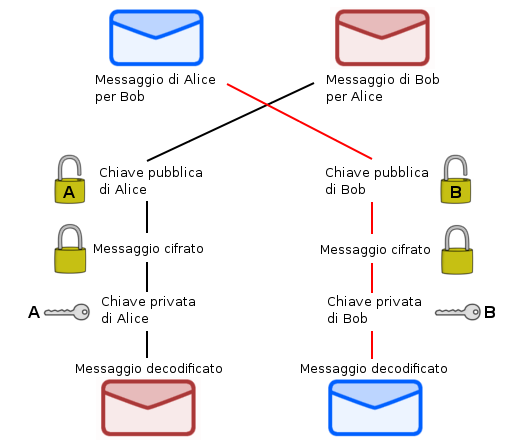
\includegraphics[scale=0.5]{pubkey-postal-analogy}
    \caption{Analogia ``postale'' della crittografia a chiave pubblica}
    \label{fig:pubkey-postal-analogy}
\end{figure}


Si pu\`o notare come per mettere in sicurezza il contenuto dei pacchi
ci sia bisogno del lucchetto del destinatario, mentre per aprirli viene
usata esclusivamente la propria chiave segreta, rendendo l'intero processo
di cifratura/decifratura asimmetrico (una chiave per cifrare ed una
differente per decifrare). Chiunque intercettasse il lucchetto (aperto)
o il messaggio chiuso con il lucchetto non potrebbe leggerne il contenuto
poich\`e non ha la chiave.

\medskip
Uno dei vantaggi della crittografia asimmetrica sta nel fatto che le
chiavi pubbliche possono essere scambiate anche utilizzando canali di
trasmissione insicuri (come ad esmpio una connessione ad Internet non
protetta). Nella crittografia simmetrica invece si rende necessario
utilizzare un canale sicuro per la trasmissione della chiave, poich\`e
l'intercettazione della stessa da parte di terzi vanificherebbe la
sicurezza del sistema stesso.

\medskip
\`E evidente che gli algoritmi asimmetrici devono essere realizzati in
modo tale da assicurare che la conoscenza della chiave pubblica e
dell'algoritmo stesso non siano sufficienti per risalire (in modo
pratico) alla chiave privata. Inoltre, poich\`e chiunque (compreso
un attaccante) \`e in grado di criptare messaggi arbitrari con la
chiave pubblica, gli algoritmi asimmetrici non devono essere
suscettibili ad attacchi di tipo ``chosen-plaintext'', in cui cio\`e
un attaccante pu\`o scegliere un messaggio (o pi\`u messaggi) in
chiaro $M$, ottenerne il rispettivo messaggio criptato $C$, e usare
questa corrispondenza per dedurne la chiave di decriptazione (o
informazioni su di essa).

\subsection{Generalit\`a e basi teoriche del crittosistem RSA}

RSA \`e un crittosistema a chiave pubblica i cui algoritmi sono basati
su semplici operazioni di aritmetica modulare (in particolare,
l'esponenziazione).

\smallskip
Il fondamento del crittosistem \`e offerto dal seguente semplice
corollario del teorema di Eulero, la cui dimostrazione \`e immediata:

\begin{corollary}\label{cor:euler-for-rsa}
Sia $n = pq$ prodotto di due primi distinti, sia $e$ un intero primo con
$\ephi{n}$, e sia $d$ il suo inverso modulo $\ephi{n}$. Allora, per ogni
intero $m$, risulta\, $m^{ed} \congruent m \mmod n$.
\end{corollary}

\smallskip\noindent
Ecco ora il procedimento con cui determinare coppied di chiavi per RSA%
\footnote{Non descriveremo con precisione gli algoritmi collegati a tale
procedimento, poich\`e essi non sono stati implementati nel nostro modulo
python.}:
\begin{enumerate}\label{enum:rsa-keys}
 \item Si scelgono due numeri primi $p$ e $q$.
 \item Si calcola $n := pq$.
 \item Si calcola $\ephi{n} =  (p - 1) (q - 1) = n - p - q + 1$.
 \item Si sceglie un intero $e$ con \,$0 < e < \ephi{n}$\, e\,
       $\gcd{e}{\ephi{n}} = 1$.
 \item Si calcola l'intero $d$ tale che $0 < d < \ephi{n}$ e
       $ed \congruent 1 \mmod {\ephi{n}}$.
 \item La coppia $(n,\,e)$ costituisce la chiave pubblica.
 \item La terna $(p,\,q,\,d)$ costituisce la chiave privata.
\end{enumerate}

Si noti che, grazie all'algoritmo di Euclide esteso, ricavare la
chiave privata a partire dalla dalla chiava pubblica \`e facile ed
efficiente. D'altra parte, come visto nella precedente sezione,
affinc\`e il crittosistema RSA funzioni, \`e necessario che il
viceversa (ossia ricavare la chiave privata dalla chiave pubblica)
sia pressoch\`e impossibile in pratica. Diremo di pi\`u a questo
proposito nella successiva sezione~\eqref{subset:rsa-properties}.

\begin{algorithm}[Criptazione e decriptazione con RSA]
I messaggi che \`e possibile criptare e/o decriptare con una coppia
di chiavi RSA $(p,\,q,\,d)$ e $(n,\,e)$ consistono degli interi positivi
$m$ con $0 \leq m < n$. Per \emph{criptare} un intero ``in chiaro'' $m$,
si calcola:
\begin{equation}\label{eq:rsa-crypt}
  c = \rem{m^e}{n}
\end{equation}
mentre per \emph{decriptare} un intero ``criptato'' $c$ si calcola:
\begin{equation}\label{eq:rsa-decrypt}
  m = \rem{c^d}{n}
\end{equation}
\end{algorithm}

La correttezza dell'algoritmo deriva facilmente dal
corollario~\eqref{cor:euler-for-rsa}.  Infatti, se $c$ \`e il
risultato della criptazione di $m$, si ha:
  $$c^d \congruent {\p{m^e}}^d \congruent m^{ed} \congruent m \mmod n$$
cosicch\`e decrittando $c$ si riottiene davvero $m$.

\subsection{RSA per messaggi binari qualunque}

Come visto nella precedente sezione, l'algoritmo RSA ``semplice'' \`e
in grado di operare solo su numer interi limitati, ossia i possibili
``messaggi'' sono tutti e soli gli interi $m$ tali che $0 \leq m < n$
(la loro massima grandezza dipende quindi dal modulo $n$ della chiave).

Tuttavia, nella pratica, si \`e generalmente interessati a criptare
generiche sequenze di bytes.  Il metodo pi\`u semplice per far ci\`o
consiste nel complementare l'algoritmo RSA con protocolli e algoritmi
in grado di convertire efficientemente input ed output binari \emph{da}
ed \emph{in} sequenze di interi di grandezza massima prestabilita
(cossicch\`e sia poi possibile criptare/decriptare questi interi uno
ad uno).

La nostra implementazione di RSA in python fornisce tali metodi, ed
offre commenti approfonditi circa il loro funzionamento. Sebbene
l'implementazione e gli algoritmi da noi scelti siano probabilmente
non ottimali, essi sono corretti, testati, e sufficienti per i nostri
scopi.

\subsection{Propriet\`a basilari di RSA}\label{subset:rsa-properties}

\TODO: conoscere uno qualunque tra $\ephi{n}$, $p$, $q$ o $d$ equivale
a conoscere tutta la chiave privata.
\\
\TODO: simmetria fra criptazione e decriptazione (utile in firme digitali).
\\
\TODO: ragionevole efficienza, dovuta all'uso
       dell'algoritmo~\eqref{alg:square-and-multiply}
       ``square and multiply'' per l'esponenziazone modulare

\medskip\noindent
Infine, la \emph{decriptazione} di un messaggio criptato con RSA pu\`o
essere velocizzata con l'uso del seguente risultato\footnote{Si noti che
la \emph{criptazione} con RSA non pu\`o sfortunatamente usufruire della
stessa ottimizzazione, poich\`e quest'ultima richiede la conoscenza dei
fattori $p$ e $q$ di $n$, il che equivale all conoscenza della chiave
privata -- che come noto non pu\`o essere resa nota al pubblico.}:
%
\begin{theorem}
Sia $n = pq$ prodotto di due primi distinti, e siano $m$, $k$ due
interi con $k > 0$.  Siano poi \,$k_p := \rem{k}{(p-1)}$,
\,$k_q := \rem{k}{(q-1)}$, e sia $x$ intero tale che
$px \congruent 1 \mmod q$., \,$m_p \congruent  \mmod p$\,
e \,$m_q \congruent m^{k_q} \mmod q$. Risulta allora
$m^k \congruent m^{k_p} + px\p{m^{k_q} - m^{k_p}}\mmod n$.
\end{theorem}
%
\begin{proof}
Poniamo $a = m^{k_p} + px\p{m^{k_q} - m^{k_p}}$.  In virt\`u del
teorema~\eqref{thm:TFA-mul-2}, per provare la tesi dobbiamo solo
dimostrare che $m^k \congruent a \mmod p$ e $m^k \congruent a \mmod q$.
Ma \`e immediato verificare che:
\begin{displaymath}
  a \congruent m^{k_p} \mmod p
    \text{\quad e \quad}
  a \congruent m^{k_q} \mmod q
\end{displaymath}
e dunque ci basta dimostrare che $m^k \congruent m^{k_p} \mmod p$ e
$m^k \congruent m^{k_q} \mmod q$. Se $p \divides m$ si ha banalmente:
\begin{displaymath}
  m^k \congruent m^{k_p} \congruent 0 \mmod p
\end{displaymath}
mentre se $p \notdivides m$, posto $k = (p - 1)t_p + k_p$ con $t_p$ intero
opportuno, si ha per il teorema di Fermat (applicato nel secondo
passaggio):
\begin{displaymath}
  m^k = \p{m^{p-1}}^{t_p} \cdot m^{k_p} \congruent 1^{t_p} \cdot m^{k_p}
      \congruent m^{k_p} \mmod m
\end{displaymath}
coicch\`e in ogni caso $m^k \congruent m^{k_p} \mmod p$. Analogamente si
dimostra che $m^k \congruent m^{k_q} \mmod q$, e la tesi \`e provata.
\end{proof}

\subsection{Un esempio basilare dell'uso di RSA}

Presentiamo qui un semplice esempio dell'uso di RSA\footnote{Questo
esempio \`e in effetti spudoratamente copiato da Wikipedia, ma visto
che \`e usato anche nei nostri test python, non ci facciamo scrupolo
a ``ripresentarlo''.}. Si noti che i parametri qui utilizzati sono
artificialmente piccoli, per evitare che dettagli e calcoli complessi
oscurino l'esposizione. Nella pratica, i parametri coinvolti hanno
in genere centinaia di cifre decimali.

Iniziamo generando una coppia di chiavi. Scegliamo innanzitutto due numeri
primi distinti $p = 61$ e $q = 53$, e calcoliamo $n = 61 \cdot 53 = 3233$
e $\ephi{n} = (61 − 1)(53 − 1) = (61 − 1)(53 − 1) = 3120$. Dobbiamo ora
scegliere un numero $1 < e < 3120$ che sia coprime con $3120$; sia dunque
 $e = 17$, che come si vede facilmente \`e primo con $3120$.

\noindent
Usiamo ora l'algoritmo di Euclide esteso per calcolare l'inverso
moltiplicativo modulo $3120$ di $17$:

\begin{displaymath}
  \begin{array}{r@{~=~}r@{\:\cdot\:}r@{~+~}r}
  3120 & 183 & 17 & 9, \\
    17 &   1 &  9 & 8, \\
     9 &   1 &  8 & 1, \\
  \end{array}
\end{displaymath}
da cui:
\begin{eqnarray*}
    1 & = & 1 \cdot 9 - 8 ~= \\
      & = & 1 \cdot 9 - \p{ 17 - 1 \cdot 9 }
      ~ = ~ 2 \cdot 9 - 17 ~= \\
      & = & 2 \cdot \p{ 3120 - 183 \cdot 17 } - 17
      ~ = ~ 2 \cdot 3120 - 367 \cdot 17
\end{eqnarray*}
e quindi $d = \p{\rem{-367}{3120}} = 3120 - 367 = 2753$.

\smallskip\noindent
Dunque la chiave pubblica \`e \,$(3233,\;17)$\, e la chiave privata
\`e \,$(61,\;53,\;2753)$.

\medskip\noindent
Possiamo ora criptare il numero $m = 65$, ossia calcolare
$\rem{{65}^{17}}{3233}$. Per far ci\`o, utilizzeremo l'algoritmo ``square
and multiply'', il che ricalca la nostra implementazione in python del
processo di criptazione RSA. Operando modulo $3233$ abbiamo:
\begin{eqnarray*}
c & \congruent\!\! &
    65^{17} = {\p{{65^2}}}^8 \cdot 65 = 4225^8 \cdot 65
    \congruent 992^8 \cdot 65 = 984064^4 \cdot 65 \congruent
  \\
  & \congruent\!\! &
    1232^4 \cdot 65 = 1517824^2 \cdot 65 = 1547^2 \cdot 65
    = 2393209 \cdot 65 \congruent
  \\
  & \congruent\!\! &
    789 \cdot 65 = 51285 \congruent 2790
\end{eqnarray*}

\noindent
Vorremo poi decriptare $c = 2790$, e verificare che il risulato \`e
proprio $m = 65$ come ci si aspetterebbe. A tale scopo dobbiamo
effettuare il pi\`u complesso calcolo $\rem{2790^{2753}}{3233}$.
Sempre seguendo da vicino la nostra implementazione python, calcoliamo
innanzitutto $\rem{2790^{2753}}{61}$ e $\rem{2790^{2753}}{53}$.

\noindent
Essendo $2790 \congruent 45 \mmod{61}$ e $2753 \congruent 53 \mmod{60}$,
operando modulo $61$ abbiamo:
\begin{eqnarray*}
m_{61}
  & \congruent\!\! &
    2790^{2753} \congruent {45}^{53} = \p{{45}^2}^{26} \cdot 45
    = 1764^{26} \cdot 45  \congruent 12^{26} \cdot 45 =
  \\
  & =\!\! &
    144^{13} \cdot 45 \congruent 22^{13} \cdot 45
    = 22^{12} \cdot \p{22 \cdot 45} = {484}^6 \cdot 990
    \congruent {57}^6 \cdot 14 \congruent
  \\
  &\congruent\!\! &
    16^3 \cdot 14 = 16^2 \cdot \p{16 \cdot 14} = 256 \cdot 224
    \congruent 12 \cdot 41 = 492 \congruent 4 \mmod{61}
\end{eqnarray*}

\noindent
Similamente, essendo $2790 \congruent 34 \mmod{53}$ e
$2753 \congruent 49 \mmod{52}$, operando modulo $53$ abbiamo:
\begin{eqnarray*}
m_{53}
  & \congruent\!\! &
    2790^{2753} \congruent {34}^{49} = \p{{34}^2}^{24} \cdot 34 =
    1156^{24} \cdot 34 \congruent 43^{24} \cdot 34 =
  \\
  & =\!\! &
    1849^{12} \cdot 34 \congruent 47^{12} \cdot 34 = {2209}^6 \cdot 34
    \congruent 36^6 \cdot 34 = 1296^3 \cdot 34 \congruent
  \\
  & \congruent\!\! &
    24^3 \cdot 34 = 24^2 \cdot \p{24 \cdot 34} = 576 \cdot 816 = 470016
    \congruent 12 \mmod{53}
\end{eqnarray*}

\noindent
Quindi, poich\`e $61 \cdot 20 - 53 \cdot 23 = 1$\footnote{Ci\`o deriva
ancora dall'algoritmo di Euclide esteso, ma questa volta omettiamo i
dettagli}, dal teorema{\XXX} ricaviamo infine:
\begin{displaymath}
  m \congruent m_{61} + 61 \cdot \p{m_{53} - m_{61}} \cdot 20
    = 4 + 61 \cdot \p{12 - 4} \cdot 20 = 9764 \congruent 65
\end{displaymath}
come ci si aspettava.

\subsection{Schemi di padding a attachi ad RSA}

When used in practice, RSA is generally combined with some padding scheme.
The goal of the padding scheme is to prevent a number of attacks that
potentially work against RSA without padding:\\
\TODO: copia da wikipedia?

LINKS:\\
~~~\verb+http://en.wikipedia.org/wiki/RSA#Padding_schemes+\\
~~~\verb+http://en.wikipedia.org/wiki/Optimal_Asymmetric_Encryption_Padding+
~~~\verb+http://en.wikipedia.org/wiki/Random_oracle_model+

%%%%%%%%%%%%%%%%%%%%%%%%%%%%%%%%%%%%%%%%%%%%%%%%%%%%%%%%%%%%%%%%%%%%%%%%%%%

\end{document}

% vim: ft=tex et ts=2 sw=2
